% this file is called up by thesis.tex
% content in this file will be fed into the main document

%: ----------------------- name of chapter  -------------------------
\chapter{An End-to-end Recurrent Neural Network Approach}\label{cp:endtoend} % top level followed by section, subsection


As recapped in Section~\ref{sec:2-rnnpm} that by now there are basically three deep learning approaches for ACE:
\begin{itemize}
\item local classification - global smoothing \cite{humphrey2012rethinking};
\item local feature learning - global classification - global smoothing \cite{boulanger2013audio,sigtia2015audio};
\item local feature learning - local classification - global smoothing \cite{zhou2015chord}.
\end{itemize}
All of these approaches incorporate a ``global smoothing'' stage after classification. This is a step that requires prior domain knowledge which does not belong to the deep learning approach itself. This chapter is going to study an ``end-to-end'' approach that tries to employ a new neural network training scheme to achieve a more balanced performance on both ordinary and long-tail chords, and on the other hand eliminate the need of ``global smoothing'' altogether. The system presented here belongs to the ``local feature extraction - global classification'' category.


%: ----------------------- contents from here ------------------------
\section{System Overview}\label{sec:4-sysover}
Figure \ref{fig:4-sysover} shows the system overview, which mainly contains a feature extraction module and a BLSTM-RNN sequence decoding module. The former is the same as the bass-treble chromagram extraction process presented in Chapter~\ref{cp:ghmm}.

\begin{figure}[htb]
\centering
\includegraphics[width=0.4\columnwidth]{4/figures/sys-chordino-like.pdf}
\caption{BLSTM-RNN end-to-end ACE System Overview. The raw audio is transformed by a feature extraction process into a piece of chromagram, and then decoded by a BLSTM-RNN into segmented chord sequence.}
\label{fig:4-sysover}
\end{figure}

\section{Implementation}\label{sec:4-blstm}
The key module in this system is the BLSTM-RNN. This section will first briefly discuss the concerns of RNN variable-length sequence training, and then elaborate on the implementation of the BLSTM-RNN.

\subsection{RNN}
A RNN can model the conditional probability of a label sequence $l$ given its corresponding input feature sequence $x$. Here let's define the label alphabet as $L$, and let both $x$ and $l$ have the same length $T$ in the unit of time. The conditional probability $p(l|x)$ modeled by the RNN can be written as:

\begin{equation}\label{eq:4-rnnprob}
p(l|x) = \prod_{t=1}^T y_{l_t}^t  \quad\quad l\in L \quad and \quad |l| = |x|
\end{equation}

where $l_t$ is the $t^{th}$ element of $l$ and $y_{l_t}^t$ is the probability of predicting label $l_t$ at time $t$ given $x$. At time $t$, $y_{l_t}^t$ can also be written as $p(l_t|x)$, which is the value of the $l^{th}$ slot of RNN prediction at time $t$. This RNN can be trained using a maximum likelihood approach by updating the network weights towards a direction that increases the conditional probability of ground truth sequences given their input representation sequences. Thus the cost function will simply be equation \ref{eq:4-rnnprob} (or the logarithm of it) given both $l$ and $x$ are in the training set.

Note that unlike ASR, training an ACE RNN using a connectionist temporal classification (CTC) cost function \cite{graves2006connectionist} is problematic and theoretically may not yield better results. This is because ACE emphasizes segmentation quality, but ASR does not. The necessity of CTC's forward and backward algorithm stems from the fact that there could be many paths that lead to the same label sequence, and this in turn is based on the fact that the length of a path could be longer than that of the label sequence. However, using CTC for transduction between two sequences of the same length will inevitably reduce the CTC cost function back to equation \ref{eq:4-rnnprob}. But this does not rule out other possible novel applications of CTC cost function to ACE, especially in combination of sequence force alignment techniques \cite{sheh2003chord,mauch2010lyrics}.

\subsection{Implementation of BLSTM-RNN}
Figure \ref{fig:4-blstm} shows the graphical model of the BLSTM-RNN, which has a forward and a backward hidden layer both with 800 LSTM units. The output layer is a \#-chord-way softmax layer, corresponding to the posterior probabilities of all classes in SeventhsBass. The input layer has 24 real-value nodes, corresponding to a bass-treble chroma.

\begin{figure}[htb]
\centering
\includegraphics[width=0.6\columnwidth]{4/figures/blstm.pdf}
\caption{The BLSTM-RNN. Both the forward and backward hidden layers contain 800 LSTM units}
\label{fig:4-blstm}
\end{figure}

\subsection{Data Augmentation}
The training/validation datasets used in this system are the same as those in Chapter~\ref{cp:ghmm}. To generate training data, firstly all raw audios are transformed to bass-treble chromagram representations. The original segment-wise ground truth annotations are up-sampled to become frame-wise annotations with 1-to-1 mappings to their input representations. Due to the absence of phase information in chromagram, all data can be circularly transposed to 12 keys to achieve 12 times data augmentation.

\subsection{Training Schemes}
A random split of 80\% of them are used as training set, and the other 20\% as validation set. During each iteration, two different training schemes are applied:
\begin{itemize}
\item completely random: one random training case is fed into an Adadelta optimizer \cite{zeiler2012adadelta} to update the network connections. Each training case contains 500 frames (subject to the end-of-track boundary condition) of audio content with ground truth labels;
\item even chance: this is inspired by the skewed class sensitive training methods \cite{chawla2004editorial}. It will be described as follows.
\end{itemize}
Considering a skewed distribution of chord classes in the training datasets \cite{burgoyne2011expert}, a random sampling scheme will inevitably draw samples based on that same distribution, which probably causes lack of exposure to long-tail chords. Therefore, the ``even chance'' scheme is invented to let each class has an equal chance to be seen during the training process. Concretely, the scheme is formalized in Algorithm~\ref{alg:4-ectrain}:
\begin{algorithm}[h]
	\caption{Even Chance Training for RNN}
	\label{alg:4-ectrain}
	\begin{algorithmic}
	\REQUIRE
	training data set - $(X,y)$;
	number of chord classes - $ydim$
	\STATE $od$ = balancedOrderedDict($y$, $ydim$)
	\STATE $iteration$ = $0$
	\WHILE {stopping criteria == \FALSE}
	\IF {mod($iteration$, $ydim$) is $0$}
	\STATE $classorderidx$ = random\_shuffle($0$:$ydim$-$1$)
	\ENDIF
	\STATE $bcidx$ = batch indexes drawn from $od$ using $classorderidx$
	\STATE update network using Adadelta optimizer with $(X,y)$ indexed by $bcidx$
	\STATE $iteration$++
	\ENDWHILE
	\end{algorithmic}
\end{algorithm}

The core of this procedure is the computation of $od$, which is a dictionary of \textit{(track index, chord change position)} indexed by chord classes:
\begin{algorithm}[h]
	\caption{balancedOrderedDict}
	\label{alg:4-bod}
	\begin{algorithmic}
	\REQUIRE
	labels of training data set - $y$;
	number of chord classes - $ydim$
	\FOR {each class $i$ from $0$ to $ydim-1$}
	\STATE initialize an empty $od[i]$
	\ENDFOR
	\FOR {each track index $j$ in $y$}
	\FOR {each frame poistion $k$ in $y[j]$} 
	\IF {$k$ is a chord change position}
	\STATE append ($j$,$k$) to $od[y[j][k]]$
	\ENDIF
	\ENDFOR
	\ENDFOR
	\RETURN
		$od$
	\end{algorithmic}
\end{algorithm}
Each entry of $od$ contains a list of \textit{(track index, chord change position)}. When drawn from the list, a random item is returned. Therefore, the $bcidx$ in Algorithm~\ref{alg:4-ectrain} contains for each class a random case in a random track starting right from the chord change position. Each case also lasts for 500 frames (subject to the \textit{end-of-track} boundary condition). This scheme guarantees an even chance of training for each class, given that each class has at least one example in the training set.

The training is regularized by dropout with 0.5 probability, and further regularized by early-stopping when there is no improvement after 10 validations, with 1000 iterations before each validation. The BLSTM-RNN is implemented and trained under Theano \cite{bergstra2011theano}. For reproducible research, the implementation of the whole system is made available online \footnote{\url{https://github.com/tangkk/tangkk-mirex-ace/}}.

\section{Results and Discussion}\label{sec:4-eval}
This section presents evaluation results of the proposed ACE approach. The test set is still the benchmarking TheBeatles180. First of all there will be a intra-comparison among variants with different configurations (Table~\ref{tab:4-varexplore}), then a comparison with Chordino will be discussed.

\begin{table}
\caption{Variations considered in this study.}
\centering
\footnotesize
\begin{tabular}{|c|c|c|} \hline
Dimension & Configurations \\ \hline
training scheme & completely random (CR); even chance (EC) \\ \hline
training data size & J; CJ; CJK; CJKU; CJKUR \\ \hline
\end{tabular}
\label{tab:4-varexplore}
\end{table}

\subsection{Overall Performance}
Table~\ref{tab:4-overallres} shows the overall results in SeventhsBass evaluation. Generally speaking, the two best variants (in terms of SB), CJKU and CJKUR, largely outperform Chordino in both SB and S, and are fairly compared with Chordino in Mm and MmB, though significantly fall short in terms of SQ.

In terms of SB, from J to CJKUR the scores increase in a diminishing way as the amount of training data increase (Figure~\ref{fig:3-SB-traindata}). Such increase is understandable since more training data leads to better generalization ability in an unknown test set drawn from a similar population. But the diminishing return is undesirable, especially for the small improvement from CJK to CJKU, and the no improvement from CJKU to CJKUR. In terms of SOSB, it is very obvious that systems with EC training have much better performances on long-tail chords. However, their SB scores are all lower than the random training scheme counterparts.
\begin{table}[htb]
\caption{Overall WCSR scores. B = Bass, Mm = MajMin, MmB = MajMinBass, R = Root, S = Sevenths, SB = SeventhsBass, SQ = Segmentation Quality; The asterisks indicate systems with even chance training.}
\label{tab:4-overallres}
\centering
\scriptsize
\begin{tabular}{|c|c|c|c|c|c|c|c|c|}\hline
System & B & Mm & MmB & R & S & SB & SQ & SOSB \\ \hline
Chordino & 76.41 & \textbf{74.30} & \textbf{71.40} & \textbf{77.19} & 52.99 & 50.60 & \textbf{83.87} & 299.01\\ \hline
J& 67.66 & 65.38 & 61.80 & 69.06 & 54.21 & 50.86 & 71.72 & 230.30 \\ \hline
J* & 68.48 & 65.05 & 61.90 & 68.96 & 53.94 & 51.10 & 71.85 & 298.42 \\ \hline
CJ & 72.59 & 68.93 & 65.49 & 72.91 & 58.33 & 55.24 & 74.20 & 288.73 \\ \hline
CJ* & 71.29 & 66.43 & 62.77 & 71.65 & 52.13 & 48.97 & 70.57 & \textbf{320.10} \\ \hline
CJK & 74.25 & 70.63 & 69.00 & 73.88 & 59.53 & 58.04 & 77.63 & 244.78 \\ \hline
CJK* & 72.05 & 67.59 & 64.70 & 72.24 & 55.29 & 53.05 & 72.21& \textbf{301.62} \\ \hline
CJKU & 74.48 & 71.04 & 69.52 & 74.16 & \textbf{61.00} & \textbf{59.65} & 76.91 & 213.67 \\ \hline
CJKU* & 72.10 & 68.93 & 67.27 & 71.68 & 57.10 & 55.63 & 74.48 & 248.65 \\ \hline
CJKUR & \textbf{76.46} & 70.33 & 68.71 & 75.98 & 60.35 & \textbf{58.92} & 76.88 & 262.48 \\ \hline
CJKUR* & 74.24 & 70.74 & 68.44 & 74.32 & 58.94 & 56.88 & 73.34 & \textbf{327.81} \\ \hline
\end{tabular}
\end{table}

\pgfplotsset{width=8cm,height=4cm,every node near coord/.append style={font=\scriptsize}}
\begin{figure}[h]
\centering
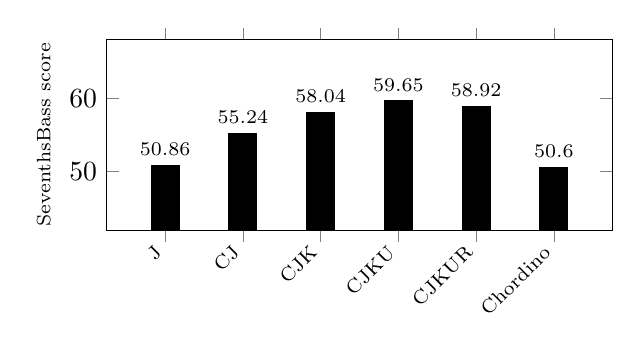
\begin{tikzpicture}
\begin{axis}[
	title= ,
	title style = {font=\scriptsize},
    ybar,
    enlargelimits=0.15,
        legend style={at={(0.5,-0.3)},
          anchor=north,legend columns=-1},
    ylabel={SeventhsBass score},
    y label style={font=\scriptsize},
    symbolic x coords={J,CJ,CJK,CJKU,CJKUR, Chordino},
    x tick label style={rotate=45,anchor=east, font=\scriptsize},
    xtick=data,
    ymin=45, ymax=65,
    nodes near coords,
    nodes near coords align={vertical},
    ]
\addplot [fill=black,draw=black] coordinates {(J,50.86)(CJ,55.24)(CJK,58.04)(CJKU,59.65)(CJKUR,58.92)(Chordino,50.60)};
\end{axis}
\end{tikzpicture}
\caption{SeventhsBass score v.s. training data size increases}
\label{fig:3-SB-traindata}
\end{figure}

%With a detail look into the per chord type results comparison among CJK, CJKU and CJKUR in Table~\ref{tab:4-detailres}, it will again be understandable. There is a small deficiency (1\%) of CJKU than CJK in terms of recognizing the dominating major triads (M), which overshadows huge improvement in minor triads (m) and dominant sevenths (7). A further discussion of the confusions and inconsistency issue may shed more light on the diminishing return.
%\begin{landscape}
%\thispagestyle{plain}
\begin{table*}[h]
\scriptsize
\caption{Detail SeventhsBass WCSR scores. M = Major, m = minor, N = no chord. The \%B row shows the composition of chords in the test dataset. The asterisks indicate systems with even chance training.}
\label{tab:4-detailres}
\begin{adjustbox}{width=1.3\columnwidth,center=\textwidth}
\begin{tabular}{|c|c|c|c|c|c|c|c|c|c|c|c|c|c|c|c|c|c|c|c|}\hline
\%B & 2.01 & 0.95 & 63.31 & 0.02 & 0.17 & 0.27 & 0.82 & 0.08 & 0.06 & 0.39 & 8.33 & 0.61 & 0.44 & 14.99 & 0.01 & 0.06 & 0.41 & 2.37 & 4.63\\ \hline
 & M/5 & M/3 & M & M7/5 & M7/3 & M7/7 & M7 & 7/5 & 7/3 & 7/b7 & 7 & m/5 & m/b3 & m & m7/5 & m7/b3 & m7/b7 & m7 & N\\ \hline
Chordino & 19.9 & 17.1 & 54.4 & 0.0 & 0.0 & 0.0 & 55.6 & 0.0 & 0.0 & 5.7 & 41.0 & 0.0 & 0.0 & 54.3 & 0.0 & 0.0 & 0.0 & 51.0 & 2.2\\ \hline
J & 11.9 & 31.7 & 62.0 & 0.0 & 0.0 & 0.0 & 22.3 & 0.0 & 0.9 & 16.9 & 2.8 & 0.9 & 0.1 & 42.2 & 0.0 & 0.0 & 0.0 & 38.6 & 3.2\\ \hline
J* & 17.5 & 30.6 & 61.1 & 7.8 & 0.0 & 0.0 & 31.8 & 0.0 & 8.7 & 39.1 & 7.6 & 2.5 & 3.6 & 40.5 & 0.0 & 0.0 & 2.7 & 44.8 & 3.4 \\ \hline
CJ & 18.9 & 34.4 & 65.8 & 0.0 & 0.0 & 0.0 & 37.6 & 0.0 & 0.6 & 31.2 & 3.6 & 0.3 & 0.0 & 52.8 & 0.0 & 0.0 & 0.0 & 43.5 & 3.0\\ \hline
CJ* & 17.2 & 24.0 & 55.3 & 0.0 & 0.0 & 1.1 & 45.2 & 0.0 & 33.0 & 44.5 & 9.8 & 3.6 & 10.5 & 56.5 & 0.0 & 0.0 & 0.0 & 19.5& 2.8\\ \hline
CJK & 9.8 & 24.4 & 72.5 & 0.0 & 0.0 & 0.0 & 25.0 & 0.0 & 0.0 & 20.4 & 2.5 & 0.0 & 0.0 & 42.5 & 0.0 & 0.0 & 0.0 & 47.7 & 3.5\\ \hline
CJK* & 14.8 & 25.1 & 61.0 & 13.1 & 0.0 & 0.4 & 41.3 & 0.0 & 0.0 & 34.0 & 14.0 & 2.1 & 4.4 & 53.8 & 0.0 & 0.0 & 5.5 & 32.0 & 3.2\\ \hline
CJKU & 9.8 & 20.5 & 71.5 & 0.0 & 0.0 & 0.0 & 9.4 & 0.0 & 0.0 & 0.0 & 21.5 & 0.1 & 0.0 & 56.0 & 0.0 & 0.0 & 0.0 & 24.9 & 3.0\\ \hline
CJKU* & 12.5 & 22.6 & 69.1 & 0.0 & 0.0 & 1.8 & 10.5 & 0.0 & 2.9 & 18.7 & 15.8 & 4.9 & 1.5 & 43.6 & 0.0 & 0.0 & 4.7 & 40.1 & 2.3\\ \hline
CJKUR & 9.6 & 25.3 & 69.8 & 0.0 & 0.0 & 0.0 & 18.1 & 0.0 & 2.3 & 18.8 & 19.4 & 0.0 & 1.7 & 59.3 & 0.0 & 0.0 & 0.0 & 38.1 & 2.5 \\ \hline
CJKUR* & 15.1 & 29.0 & 65.6 & 0.0 & 0.0 & 3.9 & 41.0 & 0.0 & 7.9 & 25.9 & 23.4 & 4.1 & 5.9 & 57.2 & 0.0 & 0.0 & 18.5 & 30.4 & 2.8\\ \hline
\end{tabular}
\end{adjustbox}
\end{table*}
%\end{landscape}

\subsection{The Random Training Scheme}
Here is a quick recap of the basic interpretation of SeventhsBass evaluation: SB score is the lowest one and reflects the true SeventhsBass performance with zero tolerance; the difference between S and SB reflects the amount of confusions (bass confusion) between root positions and inversions; the difference between MmB and SB reflects the amount of confusions (sevenths confusion) between triads ($maj$, $min$ and their inversions) and tetrads (sevenths and their inversions); and the difference between Mm and SB reflects the sum of all these confusions.

\Hsection{Confusions and Inconsistencies}
From J to CJKUR, as depicted in Figure~\ref{fig:3-bass-sevenths-confusion}, the amount of bass confusion decrease, while the amount of sevenths confusion remains at a certain level. This implies whenever an inversion gets misclassified, it is getting easier to be misclassified as a chord in a different root. As the amount of data increase, due to a random sampling training scheme, the inversions are getting marginalized by the dominating root position chords. The small classification hyperplanes that originally taken by inversions are encroached by the ever enlarging hyperplanes of the dominating classes. This is truly reflected in Figure~\ref{fig:3-csr-trainingdata-inv}, where the original good classification rates of \textit{M/5}, \textit{M/3} and \textit{7/b7} by CJ (both C and J alone contain around 20\% portion of chord inversions), are actually destroyed by the union of K and U, though this trend is reversed a little by adding R.

\pgfplotsset{width=10cm,height=6cm,every node near coord/.append style={font=\scriptsize}}
\begin{figure}
\centering
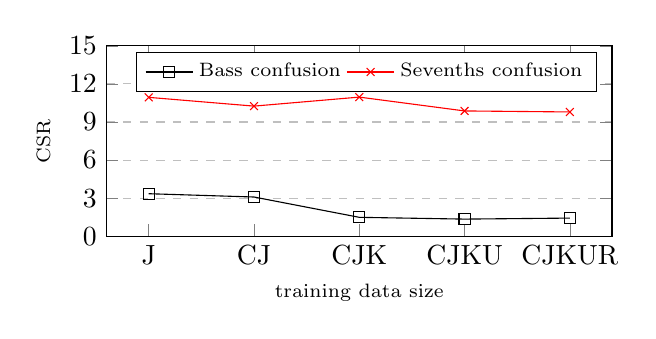
\begin{tikzpicture}
\begin{axis}[
    title={},
    title style = {font=\scriptsize},
    xlabel={training data size},
    x label style={font=\scriptsize},
    ylabel={CSR},
    y label style={font=\scriptsize},
    ymin=0, ymax=15,
    symbolic x coords={J,CJ,CJK,CJKU,CJKUR},
    ytick={0,3,6,9,12,15},
    legend pos=north east,
    legend style={legend columns=-1, font=\scriptsize},
    ymajorgrids=true,
    grid style=dashed,
]
 
\addplot[
    color=black,
    mark=square,
    ]
    coordinates {
    (J,3.35)(CJ,3.09)(CJK,1.49)(CJKU,1.35)(CJKUR,1.43)
    };
    
\addplot[
    color=red,
    mark=x,
    ]
    coordinates {
    (J,10.94)(CJ,10.25)(CJK,10.96)(CJKU,9.87)(CJKUR,9.79)
    };
\legend{Bass confusion, Sevenths confusion} 
\end{axis}
\end{tikzpicture}
\caption{Bass and sevenths confusion v.s. training data size}
\label{fig:3-bass-sevenths-confusion}
\end{figure}

\pgfplotsset{width=10cm,height=6cm,every node near coord/.append style={font=\scriptsize}}
\begin{figure}
\centering
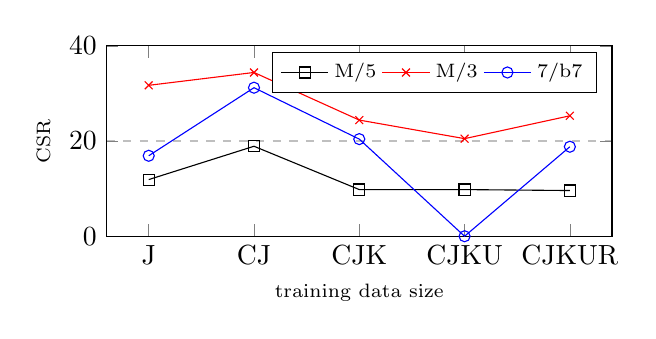
\begin{tikzpicture}
\begin{axis}[
    title={},
    title style = {font=\scriptsize},
    xlabel={training data size},
    x label style={font=\scriptsize},
    ylabel={CSR},
    y label style={font=\scriptsize},
    ymin=0, ymax=40,
    symbolic x coords={J,CJ,CJK,CJKU,CJKUR},
    ytick={0,20,40},
    legend pos=north east,
    legend style={legend columns=-1, font=\scriptsize},
    ymajorgrids=true,
    grid style=dashed,
]
 
\addplot[
    color=black,
    mark=square,
    ]
    coordinates {
    (J,11.9)(CJ,18.9)(CJK,9.8)(CJKU,9.8)(CJKUR,9.6)
    };
    
\addplot[
    color=red,
    mark=x,
    ]
    coordinates {
    (J,31.7)(CJ,34.4)(CJK,24.4)(CJKU,20.5)(CJKUR,25.3)
    };
    
 \addplot[
     color=blue,
     mark=o,
     ]
     coordinates {
     (J,16.9)(CJ,31.2)(CJK,20.4)(CJKU,0)(CJKUR,18.8)
     };
\legend{M/5, M/3, 7/b7} 
\end{axis}
\end{tikzpicture}
\caption{Inversions CSRs v.s. training data size}
\label{fig:3-csr-trainingdata-inv}
\end{figure}

\pgfplotsset{width=10cm,height=6cm,every node near coord/.append style={font=\scriptsize}}
\begin{figure}
\centering
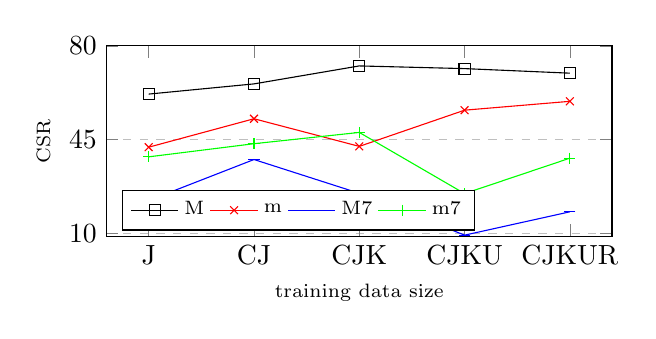
\begin{tikzpicture}
\begin{axis}[
    title={},
    title style = {font=\scriptsize},
    xlabel={training data size},
    x label style={font=\scriptsize},
    ylabel={CSR},
    y label style={font=\scriptsize},
    ymin=9, ymax=80,
    symbolic x coords={J,CJ,CJK,CJKU,CJKUR},
    ytick={10,45,80},
    legend pos=south west,
    legend style={legend columns=-1, font=\scriptsize},
    ymajorgrids=true,
    grid style=dashed,
]
 
\addplot[
    color=black,
    mark=square,
    ]
    coordinates {
    (J,62.0)(CJ,65.8)(CJK,72.5)(CJKU,71.5)(CJKUR,69.8)
    };
    
\addplot[
    color=red,
    mark=x,
    ]
    coordinates {
    (J,42.2)(CJ,52.8)(CJK,42.5)(CJKU,56.0)(CJKUR,59.3)
    };
	\addplot[
	    color=blue,
	    mark=-,
	    ]
	    coordinates {
	    (J,22.3)(CJ,37.6)(CJK,25.0)(CJKU,9.4)(CJKUR,18.1)
	    };
     \addplot[
         color=green,
         mark=+,
         ]
         coordinates {
         (J,38.6)(CJ,43.5)(CJK,47.7)(CJKU,24.9)(CJKUR,38.1)
         };
\legend{M,m,M7,m7} 
\end{axis}
\end{tikzpicture}
\caption{Sevenths CSRs v.s. training data size}
\label{fig:3-csr-trainingdata-S}
\end{figure}

However, there should not have been such drastic encroachment given that the affected classes all have distinguishable unique definitions and all their instances are consistently labeled. Therefore, the author believes the results point to a plausible, at least partial cause that these datasets are not consistently labeled. Actually, both C and J are annotated by the author of this paper, K and B are annotated in C4DM, U is annotated in NYU and R by RWC Group. As Humphrey et al. \cite{humphreyfour} point out, multiple annotators may have annotation inconsistency. This is demonstrated originally with two annotators labeling the same dataset. But this phenomenon logically also holds for multiple annotators labeling different datasets drawn from the same population.

It is estimated this is the reason behind the downgrading of $M/5$, $M/3$ and $7/b7$. Specifically, it is human annotators' disagreement on whether or not to label chord inversions, as in some scenarios, a human annotator tends to label a chord as root position regardless of the non-salient bass note (e.g., inconsistency of $C$ v.s. $C/E$), or in some other scenarios, to put a chord in root position on the bass regardless of the chord structure (e.g., inconsistency of $C/E$ v.s. $Em$ or $Em(b6)$, notably, for example, in the dynamic context of $F-C/E-Dm$ or $Dm-C/E-F$).

This also explains the up and down irregularities in the WCSR trend of $M7$ and $m7$, as illustrated in Figure~\ref{fig:3-csr-trainingdata-S}. While in this case there is only one source of ground truth inconsistency: whether or not to label a seventh extension, which is not related to the root. That is possibly the reason why the amount of sevenths confusions remains at a certain level.

\Hsection{About Dominant 7th}
Special attention is given to the $7$ chord in Table~\ref{tab:4-detailres}, where Chordino scores as high as 41\%, CJKU scores 21.5\%, and all others score less than 20\%. There is a huge gap between the baseline and the proposed systems' performances. Chordino is originally manually tuned against TheBeatles180 dataset, and that is why it gets a high score. This test set contain various song styles, including a lot of bluesy songs with progressions of \textit{dominant 7th}s. And many of these are rendered in a way with dynamic bass lines rather than static ones. But the population of $7$s in CJK, or at least in CJ, is mostly static, so that the system does not learn much about dynamic $7$s. By adding dataset U and R, which contain more examples of dynamic $7$s, the systems seem to learn and make better prediction of dynamic $7$s in the test set.

\subsection{The Even Chance Training Scheme}
As shown in Table~\ref{tab:4-overallres}, generally the incorporation of EC training downgrade the overall performances in all SeventhsBass categories, including the segmentation quality. However, it improves a lot the versatility score SOSB (Figure~\ref{fig:3-EC-SOSB}). Without using EC, none of the systems can surpass Chordino in SOSB, but with EC, two of them outscore Chordino for as many as 20 points. This can be reflected in Table~\ref{tab:4-detailres}, where systems score higher in long-tail chords such as $M/5$, $M/3$ and $7/b7$ mostly with EC than without EC. And those non-zero scores for the VERY long-tail chords, such as $m7/5$, $m7/b7$ and $m/b3$ are mostly found in EC trained entries. The major drawback of EC is that it tends to downgrade the scores of ordinary categories such as $M$ and $m$.

\begin{figure}[htb]
\centering
\pgfplotsset{width=8cm,height=4cm,every node near coord/.append style={font=\scriptsize}}
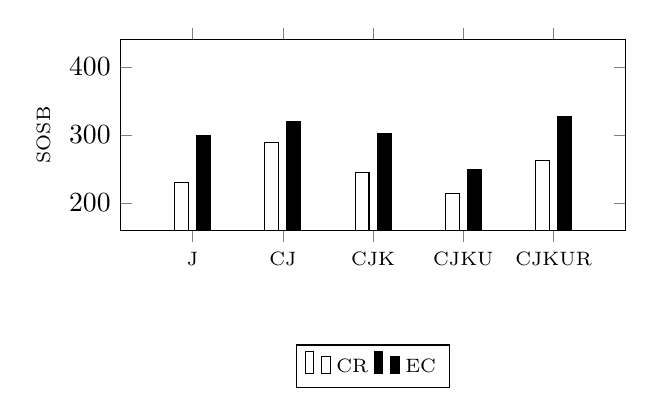
\begin{tikzpicture}
\begin{axis}[
	title={},
	title style = {font=\scriptsize},
    ybar=3pt,
    bar width=5pt,
    enlargelimits=0.2,
    legend style={at={(0.5,-0.6)},
    anchor=north,legend columns=-1},
    ylabel={SOSB},
    y label style={font=\scriptsize},
    symbolic x coords={J,CJ,CJK,CJKU,CJKUR},
    x tick label style={font=\scriptsize},
    xtick=data,
    ymin=200, ymax=400,
    %nodes near coords,
    %nodes near coords align={vertical},
    legend style={font=\scriptsize},
    ]
\addplot [ybar,fill=white,draw=black] coordinates {(J,230.30)(CJ,288.73)(CJK,244.78)(CJKU,213.67)(CJKUR,262.48)};
\addplot [ybar,fill=black,draw=black] coordinates {(J,298.42)(CJ,320.10)(CJK,301.62)(CJKU,248.65)(CJKUR,327.81)};
\legend{CR,EC}
\end{axis}
\end{tikzpicture}
\caption{Completely random (CR) training v.s. even chance (EC) training, in terms of SOSB}
\label{fig:3-EC-SOSB}
\end{figure}

\subsection{Segmentation Quality}
As illustrated in Figure~\ref{fig:3-seg-traindata}, all variants under-perform Chordino in SQ by significant amounts. They tend to improve with increasing training data size. EC training does not help SQ at all, instead, it downgrades SQ (Table~\ref{tab:4-overallres}).

Chordino segments chords by applying a very high self-transition weight in its HMM's state transition matrix. The BLSTM-RNN does not have this prior knowledge. It learns segmentation by looking at annotation changes in the training data. Unlike chord labels, segmentation information is implicit. Every training case contains 500 frames, which is about 23 seconds under our feature extraction settings. This corresponds to approximately 10-30 chord changes. Given these training cases, the BLSTM-RNN model has to learn segmentation and classification all at once. An over 77\% segmentation score is very promising indeed, but it definitely needs to be improved. A better performance could be attained by doing a dedicated training pass for segmentation only.

It is not sure why EC does not help improve SQ or at least does not affect it. Different from CR, EC training picks every cases right from the chord changes. Is it possible that such considerate practice somehow makes the machine generalize worse? Or is it because of the long-tail chords involvement? This phenomenon is yet to be understood.

\pgfplotsset{width=8cm,height=4cm,every node near coord/.append style={font=\scriptsize}}
\begin{figure}[h]
\centering
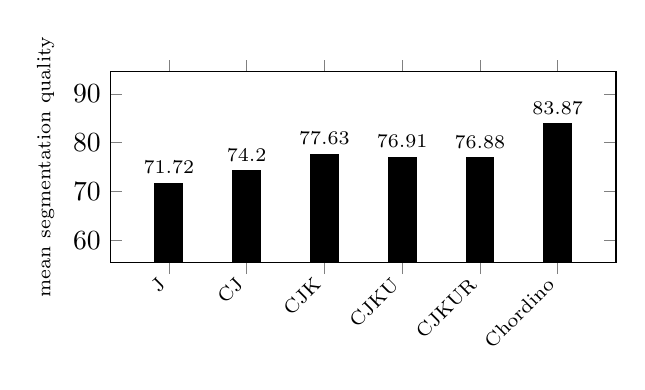
\begin{tikzpicture}
\begin{axis}[
	title= ,
	title style = {font=\scriptsize},
    ybar,
    enlargelimits=0.15,
        legend style={at={(0.5,-0.3)},
          anchor=north,legend columns=-1},
    ylabel={mean segmentation quality},
    y label style={font=\scriptsize},
    symbolic x coords={J,CJ,CJK,CJKU,CJKUR, Chordino},
    x tick label style={rotate=45,anchor=east, font=\scriptsize},
    xtick=data,
    ymin=60, ymax=90,
    nodes near coords,
    nodes near coords align={vertical},
    ]
\addplot [fill=black,draw=black] coordinates {(J,71.72)(CJ,74.20)(CJK,77.63)(CJKU,76.91)(CJKUR,76.88)(Chordino,83.87)};
\end{axis}
\end{tikzpicture}
\caption{Segmentation quality v.s. training data size increases}
\label{fig:3-seg-traindata}
\end{figure}

\section{Summary}\label{sec:4-concln}
This chapter proposes an end-to-end ``local feature extraction - global classification'' BLSTM-RNN based ACE system that supports SeventhsBass vocabulary. This system has a handcrafted feature extraction process, and can be compared with Chordino in a statistically fair way. To cater for large vocabulary recognition, an even chance training scheme is designed. Several variants of the system are trained and implemented. Evaluation results show some variants largely outperform Chordino in terms of large vocabulary scores, and they are almost as good as Chordino in terms of small vocabulary scores, despite having much worse segmentation qualities. It can be concluded that the proposed BLSTM-RNN architecture is better than the dedicated handcrafted GMM-HMM in terms of large vocabulary sequence modeling, but it suffers from bad sequence segmentation.

Through detail analysis of the results, a plausible issue of annotation inconsistency is identified. As suggested in Chapter~\ref{cp:background}, a workaround would be to always use annotations provided by one single source/annotator, or, to the other extreme, always use multiple annotators and apply majority vote or data fusion. But eventually, the ultimate evaluation tool may remain a fully subjective one, that let user experience to judge system performance.

Even chance training has been demonstrated very efficient in improving long-tail recognition accuracies. It also boosts some VERY long-tail cases from zero score to non-zero. However, it sacrifices the performances of large population chords, and thus downgrades the overall performances in all but the versatility category.

To improve this system, the key thing to be done is to improve RNN's segmentation quality, since it determines an upper-bound of all other system performance, and the scores of all other metrics scale in proportion to segmentation quality. This can possibly be done through a dedicated segmentation training pass, a deeper RNN model, or combination of a segmentation-RNN with a annotation-RNN in a hierarchical way.




% ---------------------------------------------------------------------------
%: ----------------------- end of thesis sub-document ------------------------
% ---------------------------------------------------------------------------

